% This file was created with matplot2tikz v0.5.4.
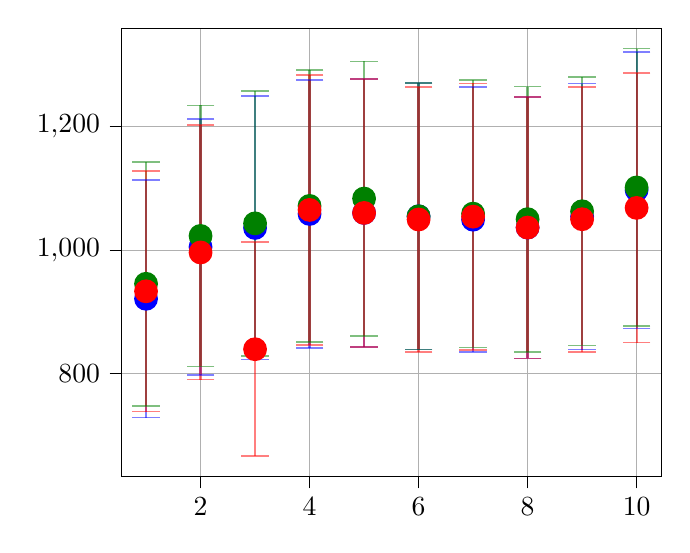
\begin{tikzpicture}

\definecolor{darkgray176}{RGB}{176,176,176}
\definecolor{green}{RGB}{0,128,0}
\definecolor{steelblue31119180}{RGB}{31,119,180}

\begin{axis}[
tick align=outside,
tick pos=left,
x grid style={darkgray176},
xmajorgrids,
xmin=0.55, xmax=10.45,
xtick style={color=black},
y grid style={darkgray176},
ymajorgrids,
ymin=633.77305, ymax=1358.80395,
ytick style={color=black}
]
\addplot [semithick, blue, mark=*, mark size=4, mark options={solid}, only marks]
table {%
1 921.241
2 1005.026
3 1035.814
4 1058.469
5 1060.114
6 1054.698
7 1049.204
8 1036.397
9 1054.171
10 1097.131
};
\path [draw=blue, draw opacity=0.5, thick]
(axis cs:1,729.117)
--(axis cs:1,1113.365);

\path [draw=blue, draw opacity=0.5, thick]
(axis cs:2,797.55)
--(axis cs:2,1212.502);

\path [draw=blue, draw opacity=0.5, thick]
(axis cs:3,822.88)
--(axis cs:3,1248.748);

\path [draw=blue, draw opacity=0.5, thick]
(axis cs:4,841.417)
--(axis cs:4,1275.521);

\path [draw=blue, draw opacity=0.5, thick]
(axis cs:5,843.068)
--(axis cs:5,1277.16);

\path [draw=blue, draw opacity=0.5, thick]
(axis cs:6,839.005)
--(axis cs:6,1270.391);

\path [draw=blue, draw opacity=0.5, thick]
(axis cs:7,834.822)
--(axis cs:7,1263.586);

\path [draw=blue, draw opacity=0.5, thick]
(axis cs:8,824.773)
--(axis cs:8,1248.021);

\path [draw=blue, draw opacity=0.5, thick]
(axis cs:9,839.068)
--(axis cs:9,1269.274);

\path [draw=blue, draw opacity=0.5, thick]
(axis cs:10,873.418)
--(axis cs:10,1320.844);

\addplot [semithick, steelblue31119180, opacity=0.5, mark=-, mark size=5, mark options={solid,draw=blue}, only marks]
table {%
1 729.117
2 797.55
3 822.88
4 841.417
5 843.068
6 839.005
7 834.822
8 824.773
9 839.068
10 873.418
};
\addplot [semithick, steelblue31119180, opacity=0.5, mark=-, mark size=5, mark options={solid,draw=blue}, only marks]
table {%
1 1113.365
2 1212.502
3 1248.748
4 1275.521
5 1277.16
6 1270.391
7 1263.586
8 1248.021
9 1269.274
10 1320.844
};
\addplot [semithick, green, mark=*, mark size=4, mark options={solid}, only marks]
table {%
1 945.484
2 1022.893
3 1043.2
4 1071.417
5 1083.349
6 1054.698
7 1058.942
8 1049.988
9 1062.776
10 1101.291
};
\path [draw=green, draw opacity=0.5, thick]
(axis cs:1,748.384)
--(axis cs:1,1142.584);

\path [draw=green, draw opacity=0.5, thick]
(axis cs:2,811.769)
--(axis cs:2,1234.017);

\path [draw=green, draw opacity=0.5, thick]
(axis cs:3,828.761)
--(axis cs:3,1257.639);

\path [draw=green, draw opacity=0.5, thick]
(axis cs:4,851.73)
--(axis cs:4,1291.104);

\path [draw=green, draw opacity=0.5, thick]
(axis cs:5,861.578)
--(axis cs:5,1305.12);

\path [draw=green, draw opacity=0.5, thick]
(axis cs:6,839.005)
--(axis cs:6,1270.391);

\path [draw=green, draw opacity=0.5, thick]
(axis cs:7,842.582)
--(axis cs:7,1275.302);

\path [draw=green, draw opacity=0.5, thick]
(axis cs:8,835.604)
--(axis cs:8,1264.372);

\path [draw=green, draw opacity=0.5, thick]
(axis cs:9,845.925)
--(axis cs:9,1279.627);

\path [draw=green, draw opacity=0.5, thick]
(axis cs:10,876.734)
--(axis cs:10,1325.848);

\addplot [semithick, steelblue31119180, opacity=0.5, mark=-, mark size=5, mark options={solid,draw=green}, only marks]
table {%
1 748.384
2 811.769
3 828.761
4 851.73
5 861.578
6 839.005
7 842.582
8 835.604
9 845.925
10 876.734
};
\addplot [semithick, steelblue31119180, opacity=0.5, mark=-, mark size=5, mark options={solid,draw=green}, only marks]
table {%
1 1142.584
2 1234.017
3 1257.639
4 1291.104
5 1305.12
6 1270.391
7 1275.302
8 1264.372
9 1279.627
10 1325.848
};
\addplot [semithick, red, mark=*, mark size=4, mark options={solid}, only marks]
table {%
1 933.323
2 996.152
3 839.673
4 1064.933
5 1060.114
6 1049.444
7 1054.067
8 1036.397
9 1049.881
10 1068.233
};
\path [draw=red, draw opacity=0.5, thick]
(axis cs:1,738.719)
--(axis cs:1,1127.927);

\path [draw=red, draw opacity=0.5, thick]
(axis cs:2,790.489)
--(axis cs:2,1201.815);

\path [draw=red, draw opacity=0.5, thick]
(axis cs:3,666.729)
--(axis cs:3,1012.617);

\path [draw=red, draw opacity=0.5, thick]
(axis cs:4,846.566)
--(axis cs:4,1283.3);

\path [draw=red, draw opacity=0.5, thick]
(axis cs:5,843.068)
--(axis cs:5,1277.16);

\path [draw=red, draw opacity=0.5, thick]
(axis cs:6,834.819)
--(axis cs:6,1264.069);

\path [draw=red, draw opacity=0.5, thick]
(axis cs:7,838.697)
--(axis cs:7,1269.437);

\path [draw=red, draw opacity=0.5, thick]
(axis cs:8,824.773)
--(axis cs:8,1248.021);

\path [draw=red, draw opacity=0.5, thick]
(axis cs:9,835.649)
--(axis cs:9,1264.113);

\path [draw=red, draw opacity=0.5, thick]
(axis cs:10,850.386)
--(axis cs:10,1286.08);

\addplot [semithick, steelblue31119180, opacity=0.5, mark=-, mark size=5, mark options={solid,draw=red}, only marks]
table {%
1 738.719
2 790.489
3 666.729
4 846.566
5 843.068
6 834.819
7 838.697
8 824.773
9 835.649
10 850.386
};
\addplot [semithick, steelblue31119180, opacity=0.5, mark=-, mark size=5, mark options={solid,draw=red}, only marks]
table {%
1 1127.927
2 1201.815
3 1012.617
4 1283.3
5 1277.16
6 1264.069
7 1269.437
8 1248.021
9 1264.113
10 1286.08
};
\end{axis}

\end{tikzpicture}
